\subsection{Machine Learning and scenario considered}

Machine Learning is the field of study that focuses on developing methods of learning general patterns from limited data. In recent years, important advances have been observed in Machine Learning research, and also the popularity and applications of some methods have increased significantly. One example is the improvement of Convolutional Neural Network architectures, and the popularity of Generative Models. Also, some recent research is focused on the theory behind such machine learning methods\cite{SAAMAP}\cite{grohs2022mathematical}, and statistical learning in general \cite{Vapnik}. Part of the goal of this formalization is to provide more qualitative guarantees in regard not only to accuracy, but also fairness, privacy, interpretability, and other important qualities. We discuss these different goals in the next four subsections.

In general, we consider \emph{supervised learning} problems: in this scenario, a \emph{machine learning algorithm} is an algorithm that receives many data points, which we call \emph{training data}, and outputs a \emph{model}. This model is itself an algorithm that receives a data point with some information omitted, encoded in what we call the \emph{target variable}, and outputs a guess of the omitted information, which we call the \emph{model prediction}. The model is then evaluated with other data points, ideally not the same ones used for training the model. This is called supervised learning because the algorithm has access to the target variable during the training process, which is not the case for unsupervised learning.

Figure \ref{fig:EEAAO} shows how the other concepts are related to machine learning in this context: we usually can assume that the training data is generated by some causal process, which can be modeled by a causal model; possible privacy attacks include performing sensitive information inference on the training data and on the model itself; we usually measure how accurate and fair a system is by analyzing its predictions for many data points; we can also obtain local and global explanations for complex models by this type of analysis.

\begin{figure*}[ht]
\centering
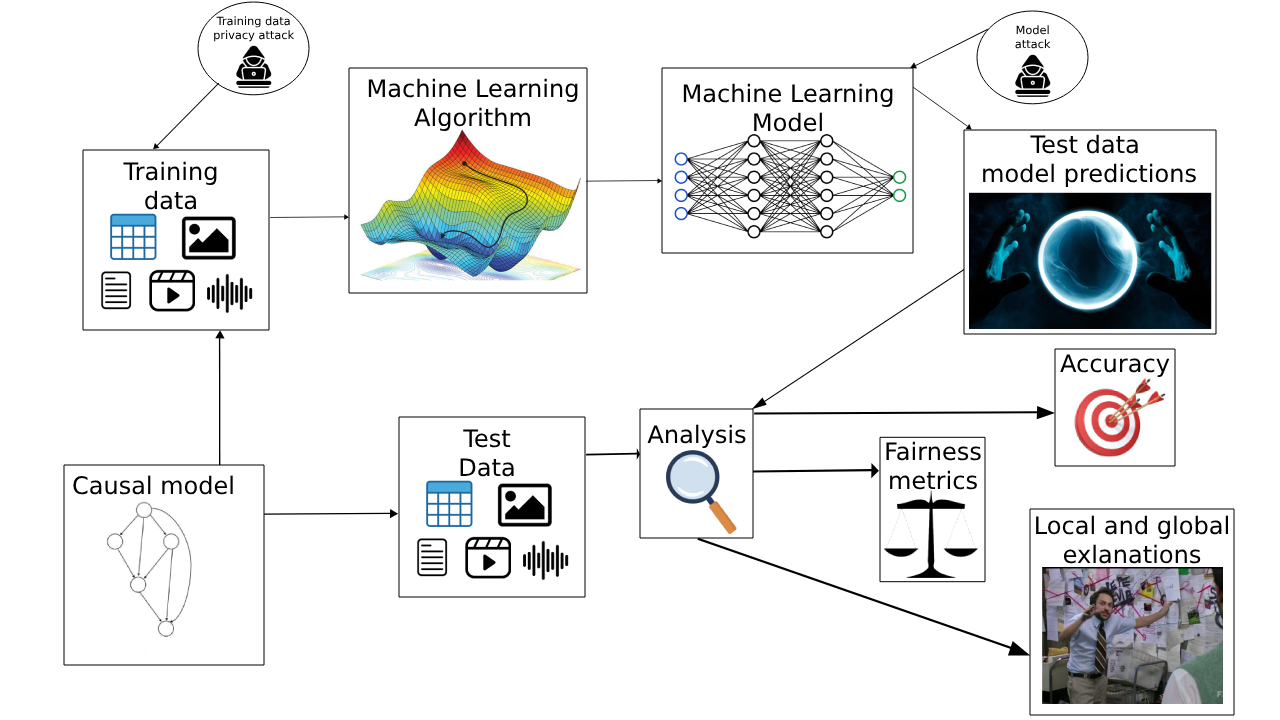
\includegraphics[width=\textwidth]{EverythingEAAO}
\caption{Figure representing the supervised learning scenario we consider throughout this work.}\label{fig:EEAAO}
\end{figure*}

\subsection{Accuracy}

\emph{Accuracy} is the notion of how close some estimate is to the true value we are estimating. In the context of Machine Learning, it represents how close the predictions of a given model are to the real value of the variable the model aims to predict. For binary classification (the scenario in which the target value has only two possible values), accuracy is defined in machine learning as $\frac{TP+TN}{TP+TN+FP+FN}$, where:

\begin{enumerate}
\item $TP$ is the number of True Positives: how many predictions were labeled as True and were really True.
\item $TN$ is the number of True Positives: how many predictions were labeled as True but were actually False.
\item $FP$ is the number of True Positives: how many predictions were labeled as False and were really False.
\item $FN$ is the number of True Positives: how many predictions were labeled as False but were actually True.
\end{enumerate}

So, the usual notion of accuracy is the proportion of the predictions from the model that were correct for the available data. This generalizes to multiclass classification problems (in which the target variable has a finite number of possible values) by considering the proportion of times that the model's prediction was the correct class. \emph{Regression} problems are the ones in which the target variable has an infinite number of possible values but can be codified as a vector of numbers: for instance, the value of some building at two different times. We can see how accurate a regression model is in many ways. For instance, by computing the square difference between the prediction value and the real value, summed for all training data points.

\begin{figure*}[ht]
\centering
\begin{subfigure}[b]{0.24\textwidth}
\centering
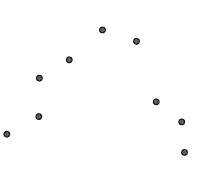
\includegraphics[width=\textwidth]{polymOverfitEmpty}
\caption{Figure representing data points.}\label{fig:polymOverfitEmpty}
\end{subfigure}
\hfill
\begin{subfigure}[b]{0.24\textwidth}
\centering
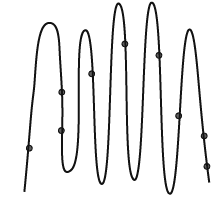
\includegraphics[width=\textwidth]{polymOverfit}
\caption{Figure representing overfitted data.}\label{fig:polymOverfit}
\end{subfigure}
\hfill
\begin{subfigure}[b]{0.24\textwidth}
\centering
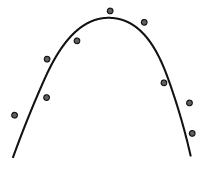
\includegraphics[width=\textwidth]{polymNotOverfit}
\caption{Figure representing non overfitted data.}\label{fig:polymNotOverfit}
\end{subfigure}
\hfill
\begin{subfigure}[b]{0.24\textwidth}
\centering
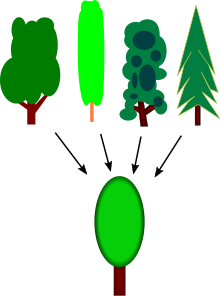
\includegraphics[width=\textwidth]{GeneralizationTreesWikipedia}
\caption{Figure representing the concept of generalization using trees. Obtained from Wikipedia.}\label{fig:GeneralizationTreesWikipedia}
\end{subfigure}
\caption{Figures representing the goal of generalization and the problem of overfitting.}
\end{figure*}

Note that during the training phase, the Machine Learning algorithm usually has the goal of providing the model that provides the best possible accuracy in the training data, among the possible models supported. If there is enough freedom among the possible models outputted from such an algorithm, then it might be possible to obtain a model that has very good accuracy, but if we try to use this same model on data other than the training data, this same model performs very badly. For instance, if we try to fit the data presented in \ref{fig:polymOverfitEmpty} with an arbitrary degree polynom, then it's possible to fit the data perfectly, as shown in \ref{fig:polymOverfit}. In this situation, the model obtained by the second-degree polynomial presented in \ref{fig:polymNotOverfit} would, in general, be more useful, even though its accuracy on the training data is not $100\%$ as in \ref{fig:polymOverfit}. This problem is called \emph{overfitting}, and is usually avoided by limiting how powerful the model can be, in conjuction with verifying accuracy values with data points not present in training dataset, which we call the \emph{testing data}. Also, note that to evaluate the model, the test data should also have the target value of each data point.


The classical goal of Machine Learning is to provide models with good \emph{test accuracy}, the accuracy evaluated for the test data, and a Machine Learning algorithm that produces models such that good results on the training data reflet on good results on testing data are said to \emph{generalize} well. The idea is that the model captures a more general abstract concept than the simple memorization of the training data, as illustrated by figure \ref{fig:GeneralizationTreesWikipedia}. 

However, note that accuracy does not always represent how accurately the model fulfills all the goals of the relevant stakeholders. This is because, with the growth of Machine Learning applications in real-life scenarios and the impact on society as a whole, there has been a growing focus on aspects other than simply maximizing the accuracy. This is similar to the way that we are sometimes worried not only about how safe a cryptographic algorithm is but also about how computationally efficient it is. 

One classical binary classification example presented in figure \ref{fig:TruePosWikipedia} is the concern with \emph{sensitivity} and \emph{specificity}: how many of the data points with target value equal to $1$ are predicted by the model to have target value $1$ and how much of the poins with target value $0$ are predicted to have value $1$ instead, respectively. One example in which this distinction is very important is in medical diagnosis: imagine that the model is predicting if someone has a deadly disease and a simple and low-risk treatment, a false negative is worse for the patient than a false positive diagnosis of having the disease. Other examples of notions to be considered, presented in \ref{fig:PrecisionrecallWikipedia}, are \emph{precision} and \emph{recall}: how many of the data points with predicted value $1$ really do have target value $1$ and how many of the data points with target value $1$ the model correctly predicted the target value, respectively. 

We can then create machine learning models that optimize for something other than accuracy. For instance, a combination of sensitivity and specificity that better suits our needs. The function that we aim to optimize with our model is sometimes called the \emph{objective function}, and we can encode many different goals in these functions, with one classical example is adding a \emph{regularization term} that penalizes more complex models, which sometimes helps in avoiding overfit.

\begin{figure*}[ht]
\centering
\begin{subfigure}[b]{0.48\textwidth}
\centering
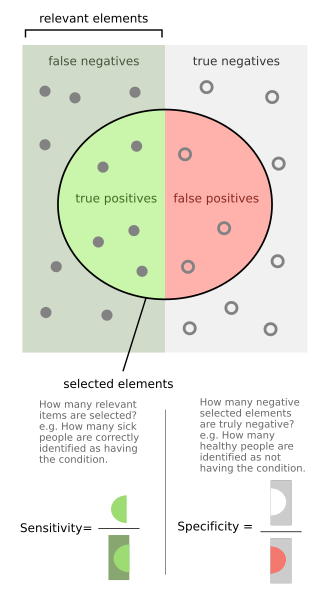
\includegraphics[width=0.6\textwidth]{TruePosWikipedia}
\caption{Figure representing the concepts of sensitivity and specificity. Obtained from Wikipedia.}\label{fig:TruePosWikipedia}
\end{subfigure}
\hfill
\begin{subfigure}[b]{0.48\textwidth}
\centering
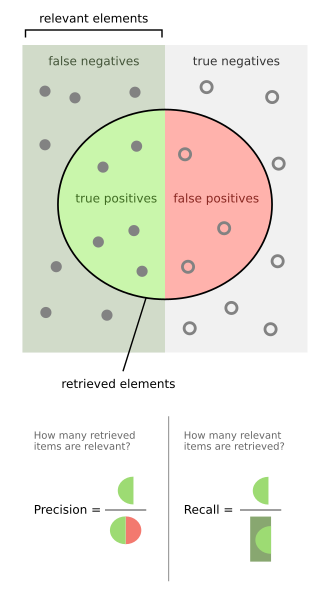
\includegraphics[width=0.6\textwidth]{PrecisionrecallWikipedia}
\caption{Figure representing the concepts of precision and recall. Obtained from Wikipedia.}\label{fig:PrecisionrecallWikipedia}
\end{subfigure}
\caption{Representation of some notions other than accuracy.}\label{fig:otherNotionsACC}
\end{figure*}

Usually, there are other important goals to keep in mind when developing a machine learning algorithm: the fairness goal aims to reduce unfair disparities in treatment of different individuals by machine learning models, the privacy goal aims to reduce the chance of someone discovering confidential or private data without authorization, and the explainability goal aims to improve the comprehension of how complex models work. Causality and Quantitative Information Flows are not goals by themselves, but methods for the representation and pursuit of other goals.

\subsection{Fairness}

In the context of Machine Learning, fairness refers to the reduction, as much as possible, of \emph{algorithmic bias}, the bias introduced by algorithmic decisions. This bias might have a big social impact because this can expand existing unfair discrimination in society, as machine learning algorithms are being used to make more and more important decisions. One famous example is the COMPAS recidivism algorithm, which has been used by the United States courts to estimate how likely someone is to reoffend in the future. It was revealed \cite{Compass} that this tool was heavily biased against black people. 

For binary classification, we will say that the result is \emph{positive} for a data point if it benefits the person represented by that data point, and \emph{negative} otherwise. We will say that the \emph{unprivileged group} is the group of people affected negatively by the bias, and the \emph{privileged group} is the other group of people.

Such biases can happen because of many factors. The algorithm itself might introduce bias, or the data might be biased. The data may have been collected in a biased way (in the COMPAS example, this would be the case if reincidivism data was collected more for black reincidivists than for white), or the data might be simply reinforcing some bias in society. 

Also, the bias in society might be such that the data is in disagreement with reality (the unprivileged group's true values for the target variable would affect them in the same way as the privileged group), or it is in agreement with reality because of structural biases in society. For instance, if the prediction of the algorithm is whether someone will have good grades if accepted to some university, people in the unprivileged group might not have had as good oportunities in life as people in the privileged group, so the data is correct when it says that those people will have worse grades. Even so, the results might still be considered unfair, this depends on the notion of fairness we consider. All of these unfairness possibilities can be further divided into other types of unfairness, as was done in \cite{mehrabi2021survey}. Image \ref{fig:whereUnfair} illustrates where unfairness might come from, and we summarize below the ways in which unfairness might be introduced:

\begin{enumerate}
\item Algorithm results do not reflect the data.
    \begin{enumerate}
    \item The algorithm might optimize for the majority only, achieving good overall accuracy even though it's mostly wrong for minorities. This can be considered a type of Aggregation Bias.
    \item Systematic errors in the algorithm, that lead to biased estimation.
    \end{enumerate}
\item The data can be biased, not reflecting the reality.
    \begin{enumerate}
    \item We can have structural biases in society, such that people in unprivileged groups do not have the necessary opportunities, but if they were treated similarly to the privileged group by society, they would have similar results. For instance, an unprivileged group that doesn't have good educational opportunities will have worse scores on exams because of historical discrimination, and although just looking at whether someone is in this group could lead to a good accuracy, it might only perpetuate current unfair biases in society.
    \item The bias can also be introduced in a way that people in the unprivileged group were misclassified before the data was collected. For instance, maybe capable people in an unprivileged group usually don't get a job even though they are actually as capable as the unprivileged group.
    \item Data collection doesn't reflect the reality: Measurement bias (for instance, COMPASS used friend/family arrests as a proxy for a risk score present in the dataset), Omitted Variable Bias (this violates assumptions of some learning models, for instance linear regression models usually assumes error terms uncorrelated with the parameters considered in the regression), Representation/Sampling Bias (biased sampling lacking the diversity of the population), Simpson's Paradox (if we don't have data on a confounder, correlations might be spurious \cite{Causality}).
    \item If the data is collected on a group fundamentally distinct from the one where it will be used, for instance another population (Population Bias) or the same population but at another time (Temporal Bias), unfair bias might be introduced.
    \item Data that relies on people's opinion is prone to many biases: Social Bias (people do what others are doing), Self-Selection Bias (people think that everyone agrees with them), and many others.
    \end{enumerate}
\item Data might depend on the algorithm's previous output: Presentation Bias (the user is presented to some selected advertisements, for instance), Ranking Bias (search engines ordering results in a biased way), Popularity Bias (more popular items are shown more). This might strengthen biases through time. 
\item Finally, the circumstances can change through time, either by the influence of the algorithm itself or other factors, which can worsen the quality of algorithms previously considered able to provide good results (Emergent Bias).
\end{enumerate}



\begin{figure*}[ht]
\centering
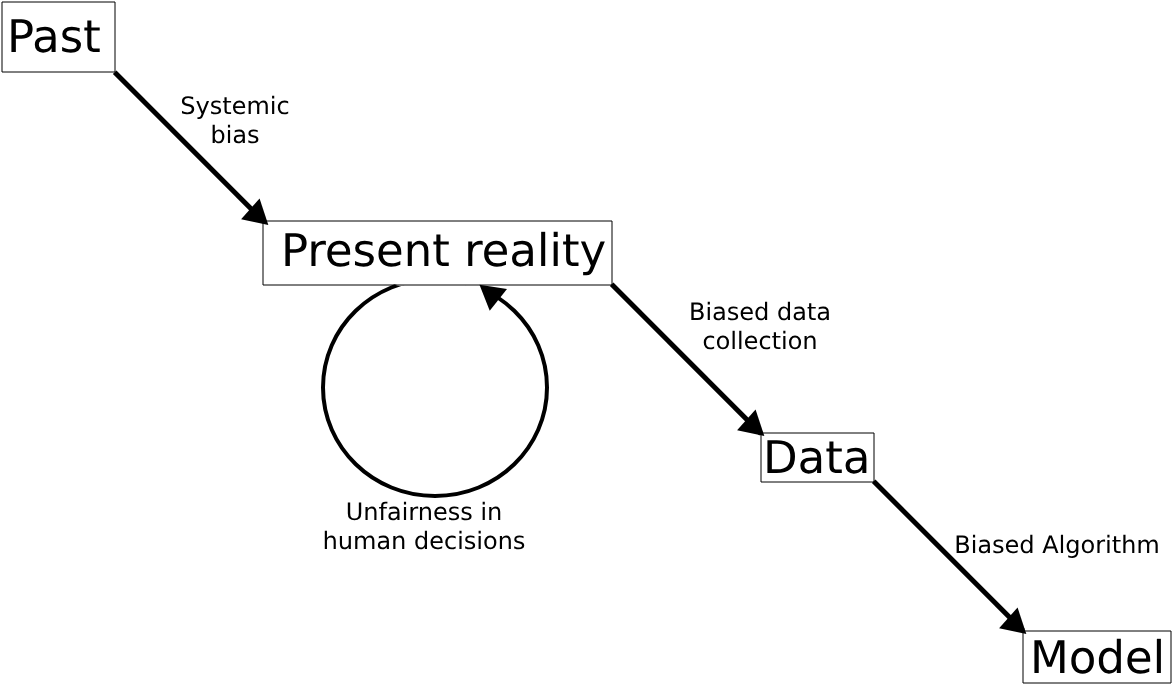
\includegraphics[width=\textwidth]{whereUnfair}
\caption{Figure representing some of the main possible sources of unfairness.}\label{fig:whereUnfair}
\end{figure*}

Besides biased data and deliberate bias in the algorithm, such that the results of the algorithm do not reflect the data, it is also possible to introduce bias because the algorithm might prioritize making correct predictions for the majority of the population, if it can't make correct predictions for both the majority and the minority. Another possibility is that the prediction might depend on past decisions of the algorithm, and we only know the result if the result provided is positive (for instance, we only know if someone will reincide if we release them). In this type of scenario, according to Learning Theory, it's important to take suboptimal decisions to \emph{explore} different options and gather more data \cite{chouldechova2018frontiers} (found in \url{arxiv.org}), which might be considered unethical as it might have a big cost to society (releasing someone that's probably going to commit more crimes) or to the individual (not giving a life-saving drug to some patients as an experiment to see the survival rates for that specific group). 

Many different notions of algorithmic fairness have been developed, and some are not compatible \cite{alves2023survey}. Initially, the notions of fairness could be grouped into two main types: statistical and individual definitions of fairness\cite{chouldechova2018frontiers}. Statistical (group) notions of fairness require some statistical metrics to be similar for certain demographic groups, and individual notions enforce constraints on pairs of individuals, for instance requiring similar individuals to be treated similarly. Many problems with statistical notions and why they, in general, don't provide good individual guarantees are presented in \cite{Awareness}\cite{kearns2018preventing}. For instance, one such problem is satisfying the constraints for two protected attributes individually but not for combinations of these attributes. One problem with both individual and group notions is \emph{composition}: it is not always the case that satisfying fairness constraints in individual, isolated, components of a system imply that fairness constraints will be satisfied for the whole system \cite{dwork2018fairness}. Finally, there are also causal approaches to fairness notions, which we will discuss more in Section \ref{sec:theoRef2}. In general, it is not possible to satisfy some of the main notions of fairness at the same time\cite{hellman2020measuring}\cite{bell2023possibility}\cite{zemel2013learning}, and which fairness notion to use depends a lot on the specific goals of each different system. We will now define some of the main notions of fairness. We consider that $Y$ is the binary target variable, with $Y=1$ as the positive result and $Y=0$ as the negative one; $A$ is the binary sensitive attribute, with $A=1$ for the privileged group and $A=0$ for the unprivileged group; $\hat Y$ is the model prediction of the target variable value; $X$ is a set of legitimate factors that can be used for classification.

\begin{definition}[Equal Opportunity Difference] We define \emph{Equal Opportunity Difference} as $P(\hat Y = 1| A = 1, Y =1) - P(\hat Y = 1| A = 0, Y = 1)$. Equal Opportunity is \emph{satisfied} if the Equal Opportunity Difference is equal to zero.
\end{definition}

\begin{definition}[Statistical Disparity] We define \emph{Statistical Disparity}, also known as \emph{Demographic Disparity}, as $P(\hat Y = 1| A = 1) - P(\hat Y = 1| A = 0)$. Statistical (Demographical) \emph{Parity} is \emph{satisfied} if the Statistical Disparity is equal to zero.
\end{definition}

\begin{definition}[Conditional Statistical Disparity] We define \emph{Conditional Statistical Disparity}, conditioned on $x$, as $P(\hat Y = 1| A = 1, X = x) - P(\hat Y = 1| A = 0, X = x)$. Conditional Statistical \emph{Parity} is \emph{satisfied} if the Conditional Statistical Disparity is equal to zero.
\end{definition}

A possible general definition of \emph{individual fairness} notions is that an algorithm is considered fair if it gives similar outcomes to similar individuals, according to similarity notions relevant to the specific scenario considered.

The techniques developed to reduce unfairness in algorithmic decision-making can be divided into \emph{pre-processing}, \emph{in-processing} and \emph{post-processing}. Pre-processing techniques modify the training data to remove biases present there. In-processing techniques modify the learning algorithm itself, for instance, by changing the objective learning function to include not only accuracy but also adding to it some statistical fairness metric, or including some constraint that it has to satisfy. Post-processing techniques act after the model is trained to reduce the unfairness in the decisions made by such a model.

In general, just removing the variables that would be considered unfair to use directly to classify an individual is not enough to guarantee fairness. As illustrated in image \ref{fig:correlated}, the variables we would remove might be highly correlated to other variables, which could be used by the model to discriminate almost as if we hadn't removed any variable. Also, even if the machine learning model itself didn't use any sensitive variables or correlated attributes for the predictions, we still need to collect this sensitive data to be able to measure how unfair the model is.

\begin{figure*}[ht]
\centering
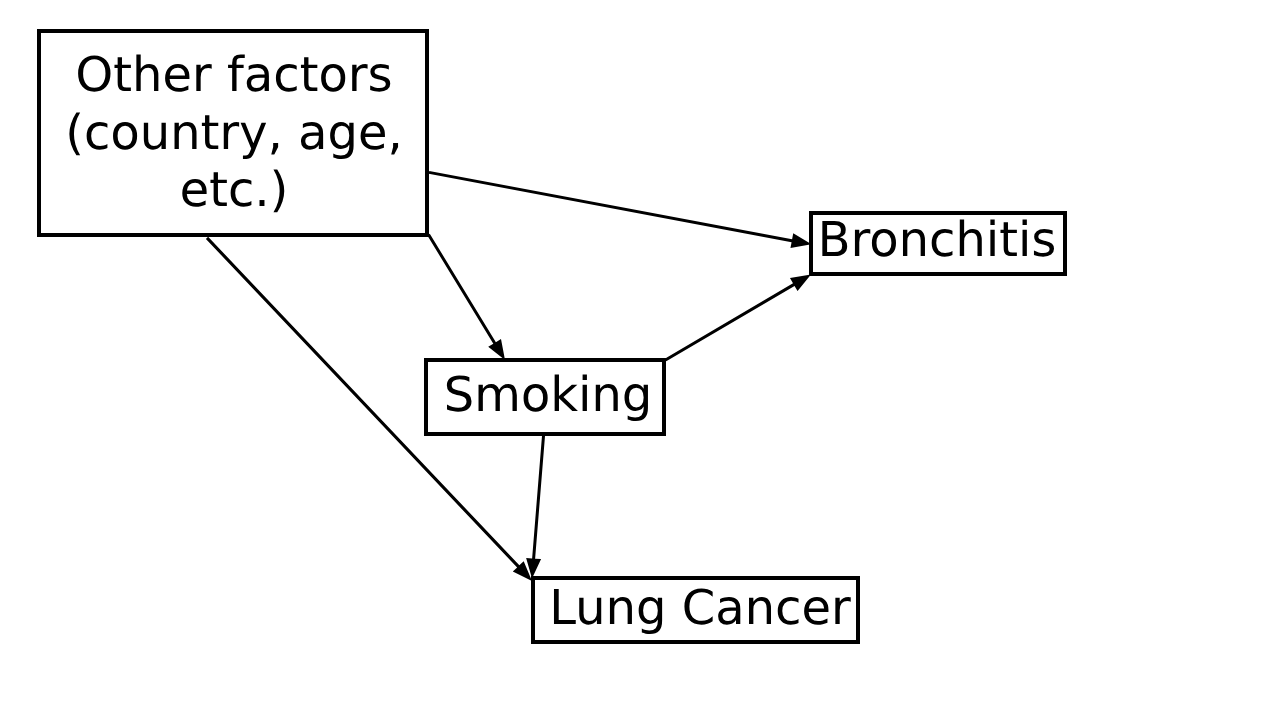
\includegraphics[width=\textwidth]{correlated}
\caption{Figure representing potential correlations between sensitive variables and other factors: if the disease status is a sensible information that could be used for unfair discrimination, then removing this information might not be enough to avoid unfair discrimination, as smoking, age and other factors combined might lead to unfair discrimination almost as if the model had direct access to the sensitive values.}\label{fig:correlated}
\end{figure*}

\subsection{Privacy}

In the context of Machine Learning, a privacy-preserving algorithm is one that does not allow information considered private/sensitive to be obtained by unauthorized parties. According to the terminology presented in \cite{liu2021machine}, this is called \emph{private ML}. The private information to be protected can be the data used to train the model or the model parameters and structure itself. It is also possible to use Machine Learning to enhance privacy, \emph{ML enhanced Privacy Protection}, or to serve as an attack tool, \emph{ML-based Privacy Attack}. We will focus on private ML.

We call \emph{adversary} the agent that wants to discover the private information, and \emph{secret} the private information itself. There are some possible goals of the adversary: she might wish to recover the model itself by trying to approximate the function that represents the model, to recover some feature or statistical property of the dataset, to discover whether some individual data point is present in the dataset, or even recover the exact values of individual samples in the dataset. We distinguish between the \emph{White-Box access} and \emph{Black-Box access} scenarios as the situation in which the adversary has or does not have full access to the trained model and their parameters, respectively. 

\emph{Model Extraction Attacks} assume an adversary with black-box access to the model, and no prior knowledge of the model parameters and training data. Some approaches to model extraction are presented in \cite{tramer2016stealing}. Although the most efficient attacks rely on confidence values, attacks that rely only on the output class labels are also presented. Other works focused on estimating hyperparameters \cite{wang2018stealing} for an adversary that knows the training dataset and the Machine Learning algorithm. Notice that recovering the model can help in the development of attacks against the training data, even if the adversary doesn't have prior knowledge of the model.

\emph{Feature estimation attacks} focus on recovering statistical properties or features of the training dataset, for an adversary that does not know the training data or the its distribution. Some attacks are presented in \cite{fredrikson2015model} both for black-box and white-box model access. As expected, the white-box attacks lead to better attacks, and they provide examples for recovering individual sensitive information from marital happiness answers in two different datasets and white-box attacks for recovering images in a face recognition model. The results lead to the possibility of (almost) identifying someone with only their name and the face recognition model and to the possibility of identifying the answer to a sensitive topic on a supposedly anonymous questionnaire (whether the person answering ever cheated on their significant other) with very high precision and a recall bigger than 20\%. 

The attacks presented in \cite{ateniese2015hacking} aims to recover statistical information about the training dataset by the use of many models trained on different datasets and a meta-classifier that identifies if a given model was trained in a dataset with some desired statistical property. This is a white-box scenario, and they focused on attacking Support Vector Machines and Hidden Markov Models. Another common type of attack is the Membership Inference Attack, reviewed in \cite{hu2022membership}, in which the adversary aims to infer whether a given data point was used to train a given model or not. One approach is presented in \cite{carlini2022membership}, in which the adversary can sample from the original data distribution and has black-box access to the target model. It works by training many \qm{shadow models} by using the data distribution, half with the target data point and half without it, then performing some computations based on confidence scores to estimate how likely the real model is to have used the relevant data point.

We will now focus on methods of protecting the training data from privacy attacks. The main methods we will mention are Differential Privacy, Local Differential Privacy, and Homomorphic Encryption.

\emph{Differential Privacy} (DP) is one of the most important definitions of quantifying privacy: the idea of DP is to define how hard it should be to distinguish one dataset from another that differs by at most any one individual data point. More generally, we can define how hard it should be to distinguish an element from a neighboring element, such that in the database example, the elements are databases and the neighboring relation is such that two databases are neighbors if and only if they differ by at most one data point. A (possibly randomized) algorithm that aims to obtain a dataset that is protected according to the DP definition is called a \emph{Differential Privacy Mechanism}. The formal definition is presented below. 

\begin{definition}[$\epsilon$-Differential Privacy] A randomized algorithm from $\mathcal{X}$ to $\mathcal{Z}$ satisfies $\epsilon$-Differential Privacy, for $\epsilon > 0$, if for every $x,x' \in \mathcal{X}$ such that $x$ is a neighgboring element of $x'$, and for every $S \subseteq \mathcal{Z}$:
$$P(\mathcal{K}(x) \in S) \leq e^\epsilon P(\mathcal{K}(x')\in S)$$
\end{definition}

The parameter $\epsilon$ can be interpreted as how close we require the probabilities of neighboring datasets to be, such that smaller values of $\epsilon$ lead to stronger requirements. In some practical applications, the Differential Privacy restriction is too strong. Thus, we have a relaxed definition for Differential Privacy, in which the parameter $\delta$ can be interpreted as the probability that the DP guarantee will not be satisfied.:

\begin{definition}[$(\epsilon,\delta)$-Differential Privacy] A randomized algorithm from $\mathcal{X}$ to $\mathcal{Z}$ satisfies $(\epsilon,\delta)$-Differential Privacy, for $\epsilon > 0$ and $\delta \in [0,1]$, if for every $x,x' \in \mathcal{X}$ such that $x$ is a neighgboring element of $x'$.
$$P(\mathcal{K}(x) \in S) \leq e^\epsilon P(\mathcal{K}(x')\in S)+\delta$$
\end{definition}

\emph{Local Differential Privacy} (LDP) is a concept important when the data collector is not assumed to be trusted and consists of the same restrictions as Differential Privacy, but with $\mathcal{X}$ as the set of possible individual values and the neighboring relation being such that all possible values are neighbors. This algorithm should be applied locally by the owner of each data point.

The idea is that individuals apply noise locally in a way such that the data collector can still obtain the desired results with the noisy data. The classical example is the scenario in which we want to discover how many people do some illegal activity (for instance, use illegal drugs) in a given region. The person answering might be tempted to lie to not let this sensitive information leak. But if we tell them to toss two coins, such that if the first one comes up heads, they answer truthfully, but if not, then the answer should be \qm{yes} if the second coin came up heads and \qm{no} otherwise. We will know that approximately $\frac{1}{2}$ of the answers is not the true answer of the person, such that half of these are \qm{yes} and half \qm{no}. We can then remove $25\%$ of the total number of answers from the number of \qm{yes} and another $25\%$ from the total number of \qm{no} to estimate the real distribution. \cite{xiong2020comprehensive} delves into many mechanisms, information metrics, and applications relevant to Local Differential Privacy, including machine learning on private data.

There are some common misconceptions about what exactly are the assumptions of Local Differential Privacy. Notice, for instance, that if the data points of two individuals are known to be highly correlated (for instance, genetic data for two siblings), then even if their data points after the application of the LDP mechanism do satisfy $(\delta,\epsilon)$-LDP, the tuple of these two data points may not satisfy $(\delta,\epsilon)$-LDP, which can improve the inferences that an adversary can make. Imagine the extreme case: if we know that all data points are equal and the LDP mechanism gives a higher probability of not changing the data point, then the adversary can discover the common value of all data points simply by looking at the most common value after the mechanism is applied. This can also be a problem for Differential Privacy, as shown in \cite{liu2016dependence}. 

The possible dependencies among data points have led to some different definitions of what exactly are the assumptions of LDP, for instance, that all data points are independent, or that the adversary knows all data points but one. \cite{tschantz2020sok} discusses how a causal interpretation can help in uncovering the meaning of each LDP assumption, which are or not equivalent, and also compares with potential causal notions of LDP. We discuss this more at \ref{sec:theoRef2}, subsection \qm{Privacy $\times$ Causality}.

\emph{Federated Learning} is another method that can help improve the privacy of individuals. The idea is that each individual trains a Machine Learning model locally, and shares information with a centralized server to improve a global model. The privacy risks are reduced because no individual data point and no individual user updates to the model are stored in the server. But still, without extra preparations, it might be possible to attack individual data points, as explored in \cite{wang2019beyond}.

Finally, \emph{Homomorphic Encryption} is a form of encryption that allows computations to be done without decrypting the data, just the result is decrypted. \emph{Secure Multi-Party Computation} is also an option if there are multiple parties responsible for this computation. The major drawback of these methods is the significant additional computational cost. Homomorphic Encryption and Secure Multi-Party Computation have been proposed for frequency estimation \cite{yang2005privacy}, Deep Learning \cite{hesamifard2017cryptodl}\cite{goswami2024privacy}, and others.

\subsection{Explainability}

Explainability, loosely defined, concerns the ability to assign meaning to why some model took one or more decisions, in a way that can be interpreted by humans. There is currently no consensus for a precise definition of the term, and many papers argue about distinctions between interpretability and explainability. For instance, \cite{gilpin2018explaining} defines interpretability as the property of being able to describe the internal working of systems to humans and \emph{completeness} as the property of being able to accurately describe the operation of the system, and an explainable system has both properties at an acceptable level. \cite{roscher2020explainable} draws this distinction differently: they define transparency as the higher-level explanation given by the designers of the system of their choices of architecture, algorithm, and hyperparameters, while interpretations are defined as answers to the question \qm{what does the model bases its decision on?}, and explanations as the combination of interpretations and contextual information from domain knowledge. In general, it is considered necessary that an explanation both explains the inner workings of a system accurately and is comprehensible enough for humans with the relevant domain knowledge. There is a trade-off between these two goals, as we want not only to reach a balance between simplicity and accuracy, but also want important biases in the model to be evident in the explanation, as mentioned in \cite{gilpin2018explaining}. This is represented by Figure \ref{fig:blackBox}.

\begin{figure*}[ht]
\centering
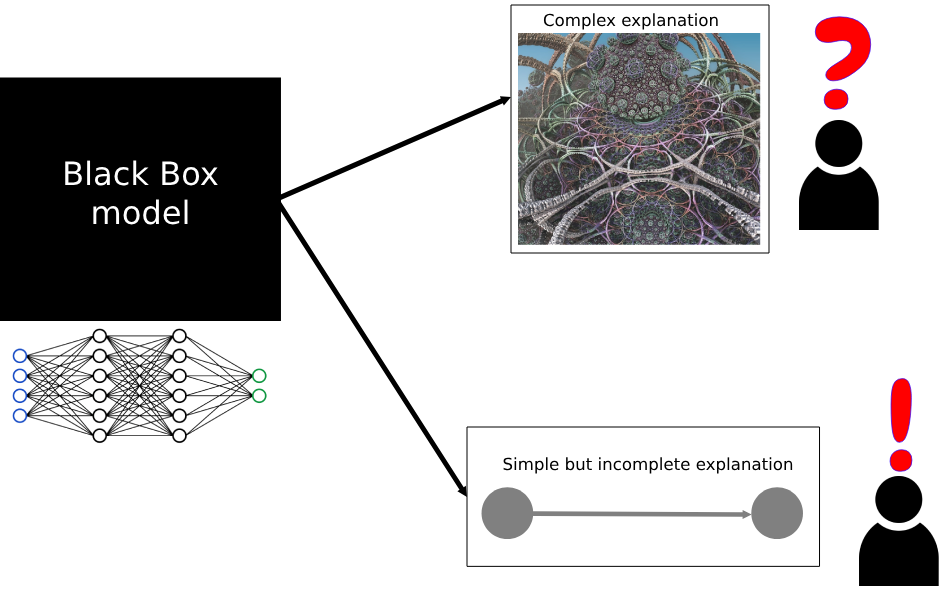
\includegraphics[width=\textwidth]{blackBox}
\caption{Figure representing two important aspects to consider when developing explanations for black-box models: how clear the explanation is for humans and how representative it is of the real model behavior.}\label{fig:blackBox}
\end{figure*}

Being able to provide good explanations for the behavior of a system has many applications, ranging from helping developers debug existing models to aiding in solving legal issues regarding whether the system is treating some minority group unfairly. There are some laws being developed to require explanations to be given when necessary, following the idea of the \qm{Right to Explanation}, under which people would be able to require exaplanations for decisions influenced by automated systems that affect their life. The European Union \qm{General Data Protection Regulation} and the French \qm{Loi pour une République numérique} are examples of laws that partially include the desired \qm{Right to Explanation}. Although the movement for requiring explanations has gained strength in the last few years, there are also arguments against requiring a comprehensible explanation to always be provided, as this might lead to a smaller accuracy than if no explanation is required, which can be harmful, for instance, for medical decisions \cite{london2019artificial}.

There are some classifications of the existing approaches to explainability, but we focus on the classification defined in \cite{linardatos2020explainable}:

\begin{enumerate}
\item We can divide the approaches based on whether they are \qm{local} or \qm{global}: \begin{enumerate}
    \item \emph{Local Explanations} focus on explaining individual decisions.
    \item \emph{Global Explanations} focus on explaining the overall workings of the model.
    \end{enumerate}
\item We can also divide the approaches into \qm{Model Agnostic} and \qm{Model Specific}: \begin{enumerate}
    \item \emph{Model-Agnostic Explanations} are methods that don't depend on the inner workings of the model.
    \item \emph{Model-Specific Explanations} refer to methods developed to work only for a specific group of models, for instance, Grad-CAM and Shap-CAM are specific for Convolutional Neural Networks.
    \end{enumerate}
\item We can divide explainability approaches based on the data types these methods deal with, for instance tabular, text, image, or graph data.
\item Finally, we can divide approaches according to the purpose of the explanations, for instance: \begin{enumerate}
    \item Creating alternative intrinsicly interpretable models.
    \item Explaining complex black-box models.
    \item Enhance how fair a model is.
    \item Test the sensitivity of predictions.
    \item Etc..
    \end{enumerate}
\end{enumerate}

LIME \cite{ribeiro2016should} and SHAP \cite{lundberg2017unified} are examples of methods that provide local explanations and can be used to derive global explanations, both are Model-Agnostic methods that deal with image, text, or tabular data, and can serve many of the explanation purposes mentioned. Figure \ref{fig:gradSHAP} shows an example of a model-specific explanation method for Neural Networks based on \qm{expected gradients}, from the \qm{shap} python package. Notice that this method shows not only what influenced the final decision, but also what influenced the model to not \qm{choose} each of the possible incorrect predictions. The model used is a Convolutional Neural Network with one output value per digit representing how much the model \qm{believes} that the input image represents that digit.

\begin{figure*}[ht]
\centering
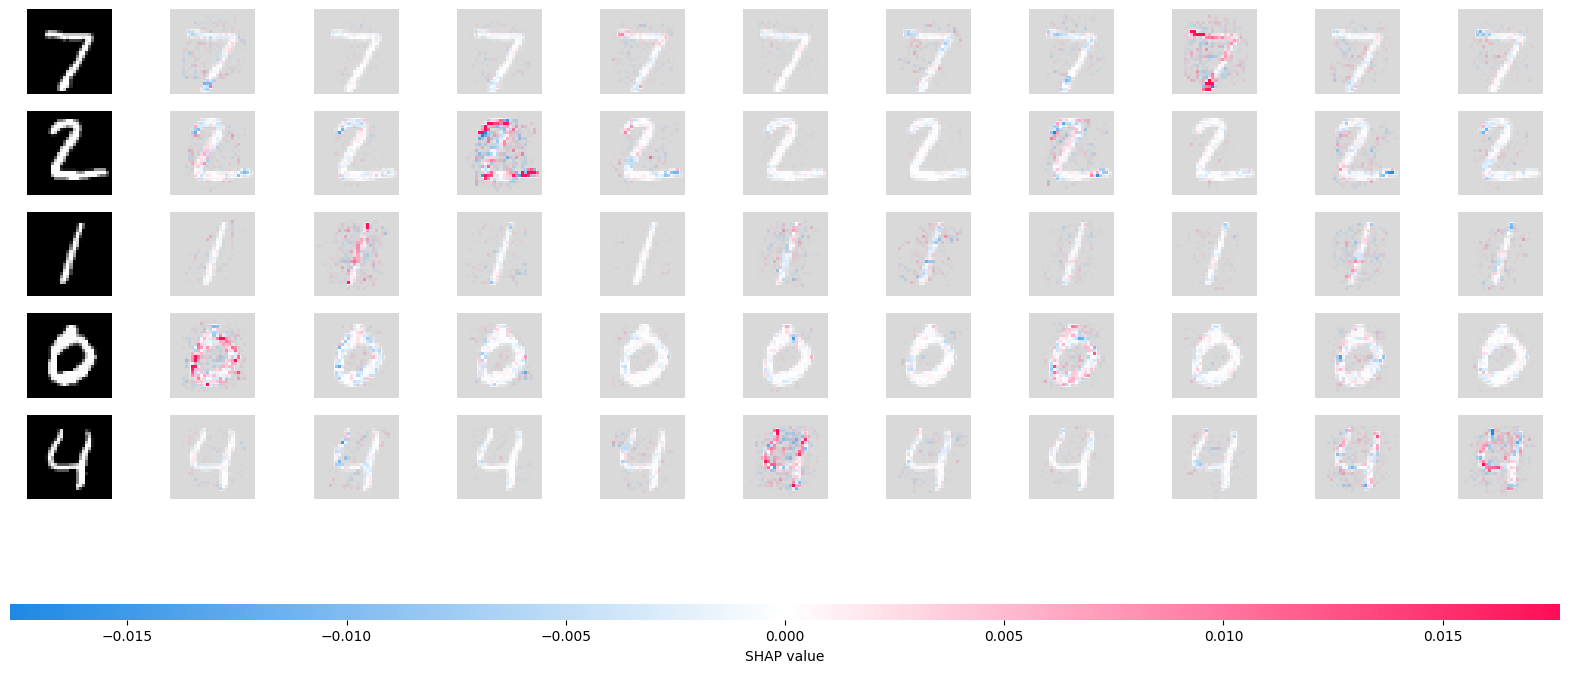
\includegraphics[width=\textwidth]{gradSHAP}
\caption{Figure representing explanations based on \qm{expected gradients} for MNIST examples, showing what pixels influenced positively (red) or negatively (blue) in the prediction. Each line represents a data point and each column a digit, such that the image in a given line and column shows which pixels influenced the output prediction of that data point representing the correspondent digit.}\label{fig:gradSHAP}
\end{figure*}

As discussed at \cite{belle2021principles}, explanations may be useful to data scientists, business owners, model risk analysts, regulators, and consumers, each with different goals in mind. The concerns that might be reduced by the use of explainable models include correctness (only variables relevant should be used in the final decisions and we should not use spurious correlations incorrectly), robustness (the model should not be susceptible to small perturbations), bias (the model should not be biased against specific subgroups), improvement (we might want to improve the model, and explanations can aid in this goal), transferability (the model should be useful in populations other than the one used to train and test the data) and human comprehensibility (this can aid an expert or even a non-expert in using and even trusting the results provided by the model).

The paper also mentions some criteria for evaluating explanations, which include how comprehensible the explanation is, how they accurately capture the models they aim to explain, how accurately they can be used to predict other outcomes of the model, how they scale to larger and more complex models, and how restrictive they are on the type of accepted model, some of these notions are further explored in \cite{carvalho2019machine}. They also evaluate explanations by example (for instance, counterfactuals \cite{verma2020counterfactual} that provide examples with small changes to an input that can modify the output), and explanations by simplification (approximating a complex model by a simpler one). These approaches are different from SHAP, for instance, as it is based on game theory-based feature importance concepts. LIME can be considered to provide explanations by simplification, by locally approximating the model to a linear model. As mentioned in \cite{roscher2020explainable}, explanations can also be used to enhance scientific research in natural sciences.

There are also inherently interpretable models, as their inner workings may be easy for humans to understand. Some examples mentioned in \cite{belle2021principles} are Linear Logistic Regression, Decision Trees, K-Nearest Neighbors (KNN), Rule-Based Learning, Generalized Additive Models (GAMs), and Bayesian Networks. Some researchers criticize this claim for some of these models, for instance, \cite{lipton2018mythos} points out that linear models are not necessarily easily interpretable, as they sometimes rely on un-interpretable and heavily-engineered features.

Other criticisms of the current development of explainability approaches were made: for instance, \cite{krishnan2020against} argues that explainability is always a means to an end, and by requiring explanations to our models we may be significantly restricting the space of possibilities of dealing with the problems we need to face. For instance, there are approaches to verify if a model is fair that does not rely on explanations of the inner workings of the model (and in this case, relying on explanations might lead to other problems, as mentioned in \cite{ExplainAll}). Another possible problem with explainability is that if we rely on human opinions we might end up with methods that are persuasive, instead of accurate, as these two properties might not be fully aligned. 

\subsection{Causality}

Most of our discussion of causality will be based on the work of Judea Pearl \cite{Causality}. There are many alternative notions of causality, but most of them are already discussed in \cite{Causality}. 

Judea Pearl divides causality into three levels (sometimes called \emph{The Ladder of Causation}), illustrated by Figure \ref{fig:levsCaus}, according to the type of question we want to answer:

\begin{enumerate}
\item \emph{The first level of causation} deals with questions that can be answered by looking at the data.  According to Pearl, this kind of question can be written in terms of what we see: for instance, given that we see that the floor of an entire street is wet then it probably rained just before. The notation used by Pearl is the usual probabilistic notation, $P(Y=y|X=x)$, abbreviated as $P(y|x)$: this means that we observed $X=x$ and want to know how likely it is for $Y$ to have the value $y$.
\item \emph{The second level of causation} concerns questions of the type: \qm{what's the consequence of some specific action}. For instance: \qm{if we make a street wet by throwing water manually into it, what is the probability that it rained?}. The difference between seeing and doing is the fundamental distinction between Pearl's first and second levels of causation. Not only is the meaning completely different, but it's also impossible to answer questions at the second level of causation by only looking at the data: extra assumptions are necessary. In our example, if we look only at the data what we see is a strong correlation between raining and the floor getting wet, and in principle, we have no idea which one causes which. There are also scenarios in which two variables are strongly correlated but neither one causes the other. For instance, in some places, the number of ice cream sales is strongly correlated with the number of deaths by  shark attacks, but clearly, that's because the times of the year when more people go to the beach are the same as when people buy more ice creams. The notation used by Pearl is $P(Y=y|do(X=x))$, which can be abbreviated as $P(y|do(x))$ or $P(y|\hat{x})$, which can be interpreted as how likely $Y$ is to have value $y$ when we set the value of $X$ to $x$ manually, and when we say \qm{manually}, we mean by an external intervention, that is not causally affected by the variables in the system. 
\item \emph{The third level of causation} regards questions of the type: \qm{what would have happened had something been different?}. For instance, \qm{what would be the average temperature of Earth had the Industrial Revolution never happened?}. Note that we observe something that happened, and then we think what would have happened if we changed something that already happened. This is what Pearl calls a counterfactual question: it requires imagining alternative worlds. To deal with this kind of question, Pearl proposes \emph{Structural Causal Models} (SCMs), which consider deterministic relationships between variables and add all the uncertainty to the values of unobserved variables. The notation used by Pearl for the counterfactual notion is $P(Y_{x'} = y| X=x)$, which can be interpreted as how likely it is for $Y$ to have value $y$ in the world that we manually set $X$ to $x'$, given that we observed that the value of $X$ is $x$. 
\end{enumerate}

Although the examples for the first level of causation usually involve some form of conditional probability, Pearl states that anything that can be computed from the joint distribution belongs to the first level of causation. This includes basically all of the usual machine learning approaches. 

Pearl claims that any method of solving questions at the second level of causation must rely on assumptions beyond the data. One way of structuring many of the relevant assumptions is by using a directed acyclic graph in which each vertex is a variable and each edge represents the causal directions between two variables. Many other types of assumptions can be made, Pearl discusses them in detail at \cite{Causality}.

Also, in the way that Pearl defines counterfactuals, there is a fundamental distinction between counterfactuals and actions with observations: in his notation, when we write the probability of some variable reaching some value given that there was an action and an observation, we interpret this as if the observation came after the action. This is different from the counterfactual notation, in which the observation comes before the action. This means that $P(Y_{x'} = y| X=x)$ is different from $P(Y=y|do(X=x'),X=x)$, as the latter should be interpreted as the probability that $Y$ has a value $y$ when we manually set $X$ to $x'$ and then observe that $X$ has value $x$, which doesn't make sense if $x \neq x'$ (we shouldn't be able to condition on impossible scenarios). This difference of interpretation can lead to confusion and was mentioned in the second part of the \qm{question to author} at \cite[Subsection~11.7.2]{Causality}.

\begin{figure*}[ht]
\centering
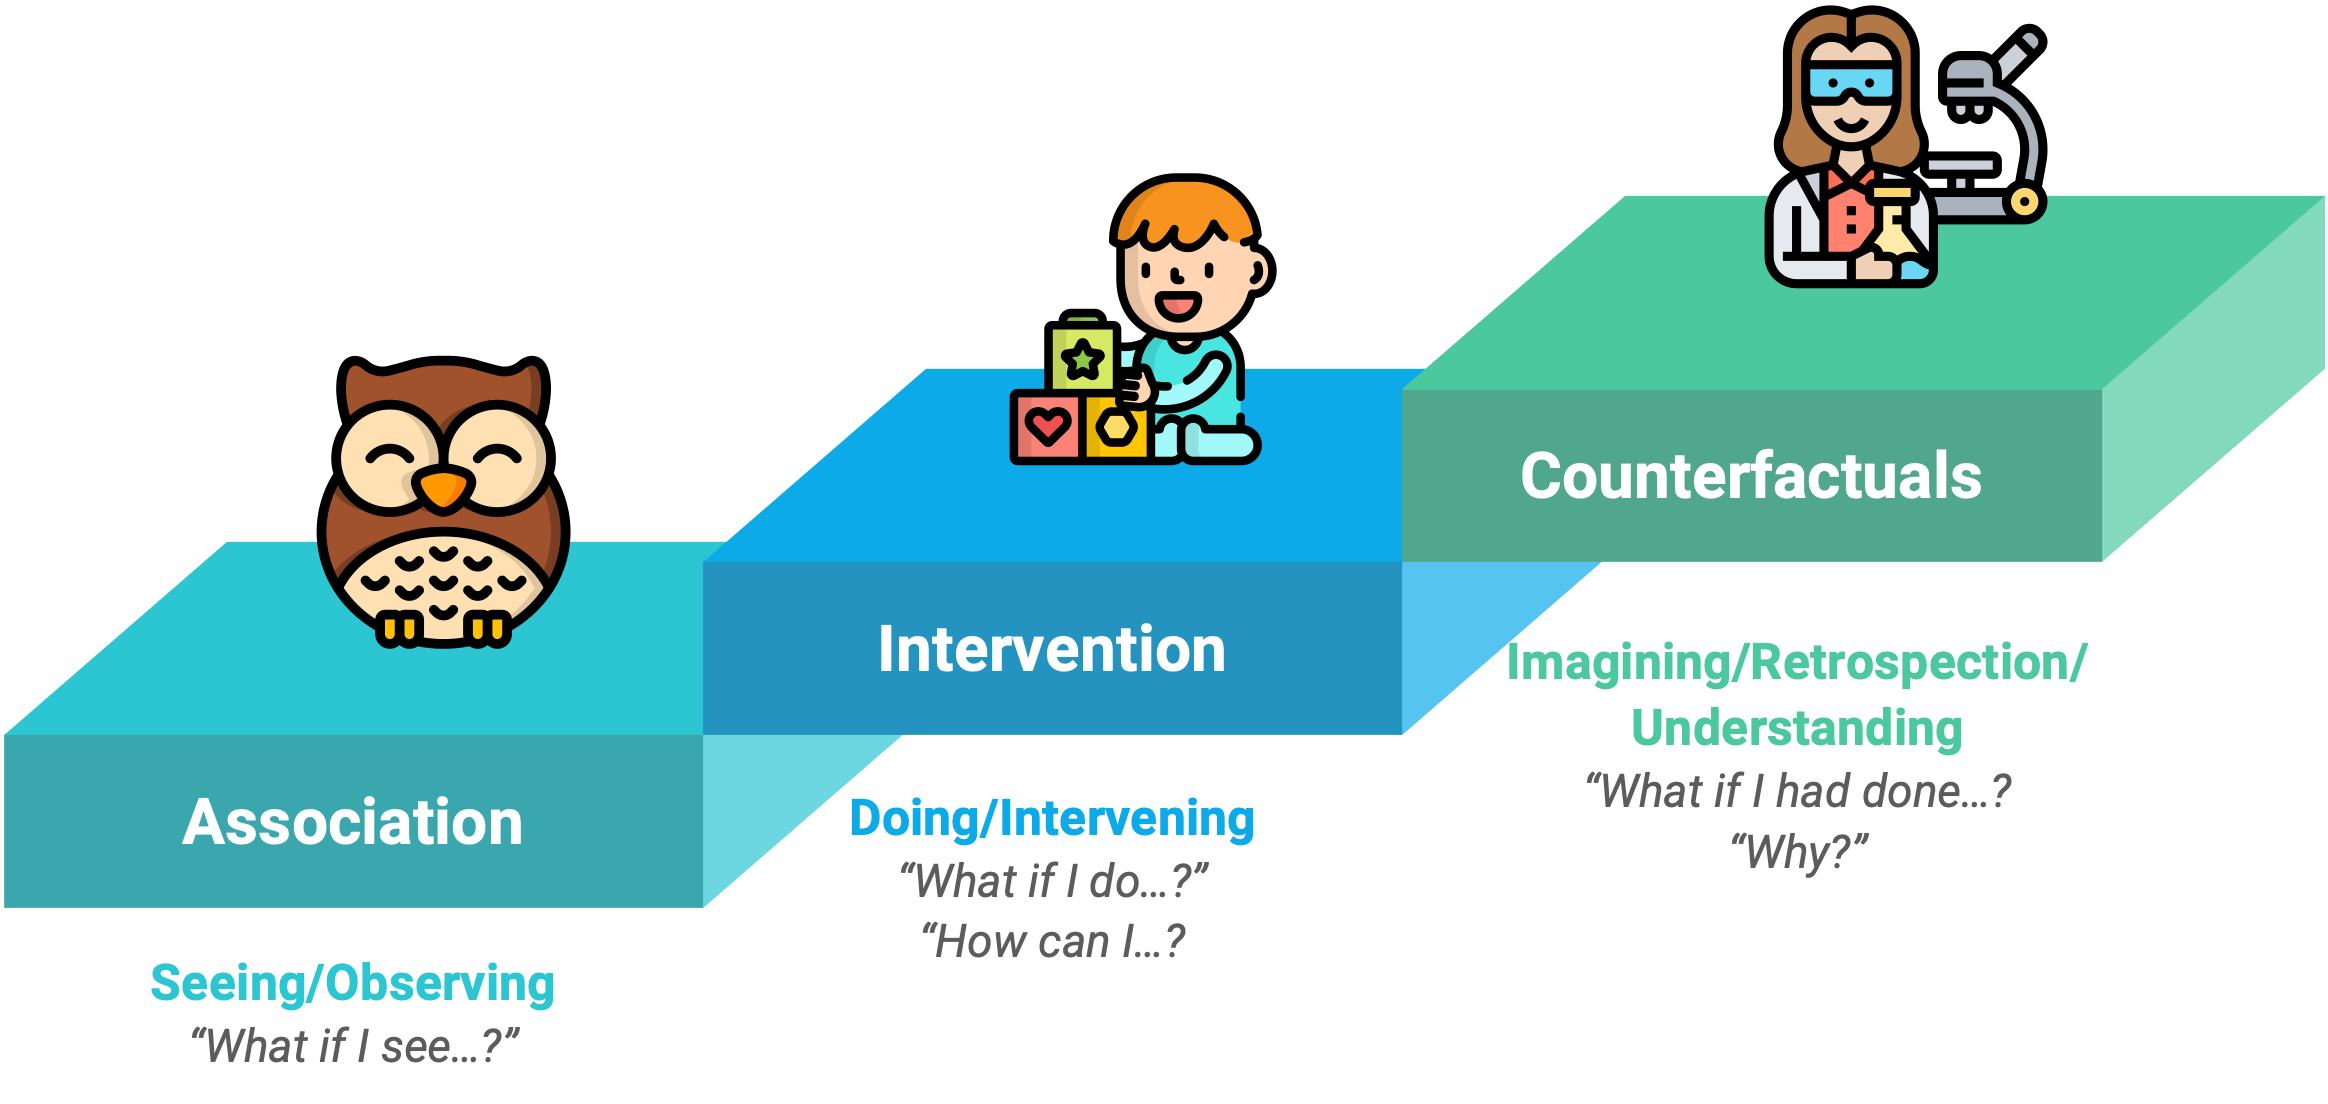
\includegraphics[width=\textwidth]{levsCaus}
\caption{Figure representing the three levels of causation.}\label{fig:levsCaus}
\end{figure*}

In general, Judea Pearl's approach to causality assumes a Directed Acyclic Graph (DAG) for the relations between variables. This leads to what is called \emph{Recursive Models} in \cite{Causality}. Many results apply only to this type of model, but some generalizations are available and mentioned in \cite{Causality}. Non-recursive models can be used for representing feedback loops: for instance, price and demand in economic models. This type of model has been widely used in economics in the form of Structural Equations, as presented in \cite[Subsection~1.4.1]{Causality}. Pearl also argues extensively about the possible causal interpretation of such equations and defines Structural Causal Models as models in which each variable has an equation that determines its value. This type of model can be used for answering questions at the third level of causation.

We will now discuss \qm{Causal Discovery} and \qm{Causal Inference}, concepts illustrated by Figure \ref{fig:discInf}.

Pearl presents many theoretical results about \emph{Causal Discovery} on \cite[Chapter~2]{Causality}, which revolves around the discovery of causal relations when we have access only to data. If two causal structures are capable of generating the same joint distributions, then we will be unable to distinguish between them if we observe only data. Also, sometimes a distribution is unstable for some models, in the sense that although the model can generate this distribution, it can only do so for some very specific configuration of the parameters. For instance, if we have $A$ and $B$ as the outcome of two independent fair coin throws ($1$ if heads and $0$ otherwise, for instance), and $C$ as the XOR between them. In the resulting joint distribution of the three variables, each pair of variables will be marginally independent but dependent if we condition on the third variable. This can be generated by three different causal structures, but only one is stable to small changes in the model (for instance, to small changes in the probability of each coin). 

With the assumption that the observed distribution is stable in respect to the underlying causal model, and based on the principle of Occam's Razor, Pearl proceeds to define algorithms to recover as much information as is possible with only the data. In general, it is impossible to distinguish some relations: for instance, $A \rightarrow B$ (meaning that $A$ causes $B$) is indistinguishable from $A \leftarrow B$ or $A \leftarrow U \rightarrow B$ for an unobservable $U$, as all three of them can generate exactly the same distributions on $A,B$ in a stable way, depending on the model's parameters. Notice that $A \leftarrow U \rightarrow B$ can also generate distributions in which $A$ and $B$ are independent: we can, for instance, set $U$ as the result of a fair four-sided dice with values $\{0,1,2,3\}$, $X$ as an indicator variable of the parity of the result ($1$ if it is odd and $0$ if it is pair) and $Y$ as an indicator of whether the result is bigger than $1$ ($0$ if it is not, $1$ if it is), in this case $X$ will be independent of $Y$ even though there is an unobservable confounder $U$. But this is not stable, in our example if we change slightly the probability distribution of $U$, for instance by increasing the probability of the outcome $0$ and decreasing all others equally, then $X$ and $Y$ become dependent, $P(X=0|Y=0) \neq P(X=0)$. Pearl provides an extensive analysis of stability and how causal relations are reflected as statistical dependencies between variables in the data.

\emph{Causal Inference} regards the problem of inferring attributes of a causal model given its structure. In this situation, we have some causal model a priori and want to estimate quantities such as $P(Y=y|do(X=x))$. Pearl introduces the \emph{$do$ calculus}, which provides a way of deriving expressions for such quantities that do not contain $do$ operator and can thus be estimated from data. The $do$ calculus is based on three basic inference rules, which were shown to be necessary and sufficient, in the sense that a causal effect based on the $do$ operator is identifiable by observing only the data and the assumption of the DAG structure of the underlying model if and only if we can derive an expression without the $do$ operator using only these three rules. Many other quantities can be defined with Pearl's framework, for instance, there are also definitions for identifying the results of dynamic plans, in which one action comes after others and might depend on the results of previous actions, which is further discussed in \cite[Section~4.4]{Causality}. 

In \cite[Section~4.5]{Causality}, Pearl dives into two other causal concepts: \emph{Direct and Indirect Effects}, which regard the effects that some variable $X$ have on another variable $Y$ that do or do not depend on other variables. For instance, smoking causes tar deposits in the lungs and also cancer, but we can think of how much of the effect of smoking on the probability of cancer is due to tar deposits, and how much is due to other factors. \emph{Natural Direct Effects} are \qm{average} estimations of direct effects for the different values the variables can assume, as the way that Pearl defines Direct and Indirect Effects is dependent on the exact values of the variables in question.

\begin{figure*}[ht]
\centering
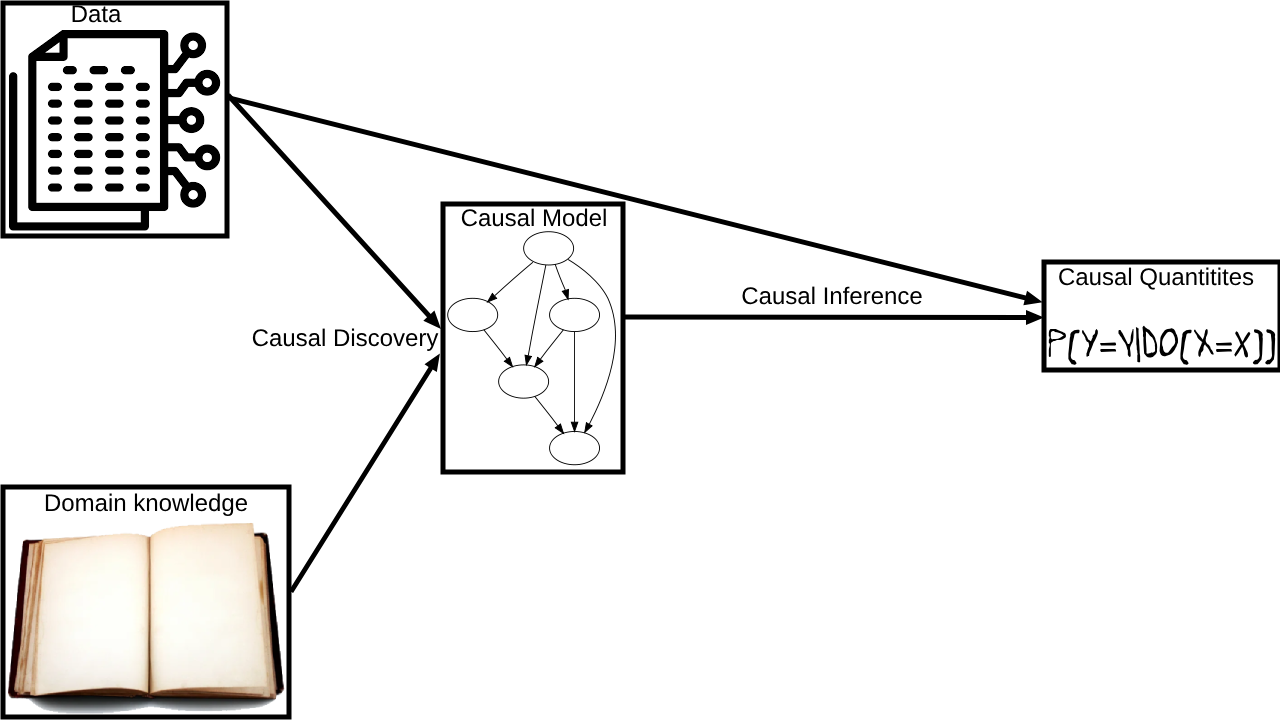
\includegraphics[width=\textwidth]{discInf}
\caption{Figure representing the difference between causal Discovery and Causal Inference.}\label{fig:discInf}
\end{figure*}

Another contribution of the causality framework presented in \cite{Causality} is the causal approach to \emph{confounding}. In some situations, it is necessary to condition on some variables to account for possible spurious correlations that might arise due to confounding, but in other situations controlling for some variables would actually create new spurious correlations. This also depends on what we want to compute, but if the goal is computing the effect of some intervention, then the $do$-calculus can be used. Pearl argues in \cite[Chapter~6]{Causality} in favor of the causal approaches to confounding.

\emph{Counterfactual statements} are defined in terms of simpler axioms, \cite[Chapter~7]{Causality} further discusses many results about counterfactuals. These results include how to use a Structural Causal Model to estimate the value of counterfactual statements, or how to check if this is even possible to estimate only with the SCM and data. \cite[Chapter~8]{Causality} delves into the problem of bounding values of expressions that can not be computed exactly. Pearl also discusses how some extra assumptions and tools can help in the estimation of expressions with the $do$ operator and counterfactual expressions: for instance, some causal quantities are easier to estimate if we can experimentally change the value of some variables via external interventions.

Finally, there are some subtleties to the meaning of causation in different settings. Pearl discusses many notions of causation besides the ones we already discussed (such as direct and indirect effects), including:

\begin{enumerate}
\item We say that $X=1$ was a \emph{sufficient cause} of $Y=1$ if when we are in a situation in which $X=0$ and $Y=0$ we expect that manipulating the value of $X$ so it becames $1$ is likely to change the value of $Y$ to $1$. In Pearl's notation $P(Y_{X=1}=1 | X=0, Y=0) \approx 1$, and $P(Y_{X=1}=1 | X=0, Y=0)$ is called the \emph{Probability of Sufficiency}.
\item We say that $X=1$ was a emph{necessary cause} of $Y=1$ if when we are in a situation in which $X=1$ and $Y=1$ we expect that manipulating the value of $X$ so it becomse $0$ is likely to change the value of $Y$ to $0$, in Pearl's notation $P(Y_{X=0}=0 | X = 1, Y = 1) \approx 1$, and $P(Y_{X=0}=0 | X = 1, Y = 1)$ is called the \emph{Probability of Necessity}.
\item There is also the \emph{Probability of Necessity and Sufficiency}, defined as the chance that manipulating the value of $X$ so it becomes $1$ will set $Y$ to $1$ and manipulating $X$ so it becomes $0$ will set $Y$ to $0$, written as $P(Y_{X=1}=1,Y_{X=0}=0)$. 
\item Pearl also defines the \emph{Probability of Disablement} as $P(Y_{X=0}=0|Y=1)$.
\item The \emph{Probability of Enablement} is defined as $P(Y_{X=1}=1|Y=0)$. 
\end{enumerate}

Many relations between these values, bounds, and conditions for identification are presented in \cite[Chapter~9]{Causality}.

The notion of \qm{Actual Cause} is defined as an alternative to the sufficient and necessary notions of causation. Pearl mentions that necessary causation is closer to \emph{token-level}, more individual than generic, as it conditions on events that really happened, while sufficient causation is closer to \emph{type-level}, more generic than individual, as the events we condition on are less specific and related to an alternative imaginary scenario. The \qm{Actual Cause} is intended to be token-level, to define what actually caused something. It is defined in terms of \qm{Causal Beams} and \qm{Sustenance}. 

We say that $X=x$ \emph{causally sustains} $Y=y$ in $U=u$ (representing the uncertainty, the unobservable factors) relative to contingencies in $W$ if and only if: $X=x$ and $Y=y$ under $U=u$; for any $w$ we get $Y=y$ under $U=u$ and interventions that set $X=x$ and $W=w$; and we get $Y=y' \neq y$ under $U=u$ and interventions that set $X=x',W=w'$ for some $x' \neq x$ and some $w'$. In other words, $X=x$ causally sustains $Y=y$ in the circumstances $U=u$ relative to $W$ when $X=x$ and $Y=y$ in the scenario $U=u$, the value of $Y$ never changes if we change the value of $W$ and keep the value of $X$, and the value of $Y$ can change if we change the values of $X$ and $W$, keeping everything else as it is with $U=u$. This means that in the situation that actually happened $U=u$, then $X=x$ is enough to sustain $Y=y$ under interventions on $W$, but if we intervene to change $X$ there will be a scenario in which intervening in $W$ changes $Y$. If $W=\emptyset$, then $X=x$ causally sustains $Y=y$ in $U=u$ relative to $W$ if in $U=u$ we have $X=x$ and $Y=y$, but it is possible to change $Y$ by changing $X$.

A \emph{Causal Beam} is a causal model defined in terms of circumstances $U=u$ and another causal model, such that the parents of each node in the new model are sufficient to maintain the value of the node regardless of the value of changes on the other parent's values, and that it is possible to change the value of other parents and the new parents to change the value of the node. If changing the value of only the new parents is enough to change the value of the node for every node, then the Causal Beam is considered a \emph{Natural Beam}. Natural Beams represent the simplified version of the model that represents the actual scenario $U=u$, such that the parents of each node are enough to sustain the value of the node regardless of changes in other variables, and are also capable of changing the value of the node by themselves. 

Pearl notes that in the definition of Causal Models provided, the parents of a node are defined in a way that makes the functions of the model non-trivial regarding all their arguments and all possible circumstances $u$, but when we consider a specific value of $U$ we can simplify the model further. The example introduced by Pearl considers $f_i(x_1,x_2,u) = ax_1+bux_2$ as the function that defines the value of variable $V_i$ in the original model: in this scenario when $u=0$ the value of $X_2$ becomes irrelevant, so we can simplify the model by defining $f_i(x_1) = ax_1$. The variable $V_i$ will then have only $X_1$ as a parent, instead of both $X_1$ and $X_2$. 

Finally, we say that $X=x$ is an \emph{Actual Cause} of $Y=y$ in the state $U=u$ if and only if there is a natural beam under circumstances $U=u$ such that if intervene with $X=x$ then $Y=y$ and if we intervene with $X=x'$ for some $x'\neq x$ we get $Y \neq y$. This represents token-level causation, whether or not $X=x$ actually caused $Y=y$ in the real scenario $U=u$. As with many of the results presented, these definitions assume we have a full description of the causal model. The notion of Actual Cause is further discussed in \cite[Chapter~10]{Causality}.


\subsection{Quantitative Information Flow}

The area of Quantitative Information Flow deals with methods of measuring information leakage from systems. This estimation is important to consider when developing real systems, as some information leakages are acceptable. For instance, whenever someone tries to authenticate with a username and password, but incorrectly guesses the password, some information leaks about the real value of the password: we now at least know that it's not the one that they tried. But we usually agree that this is acceptable while revealing the real password whenever someone makes an incorrect guess is unacceptable. How to adequately quantify the amount of information leaked from a system might depend on the goals of the people involved and on the information they have before the system executes. We thus need to first define some important notions, illustrated by Figure \ref{fig:channelAndFriends}, before proceeding:

\begin{enumerate}
\item \emph{Adversary} is an agent that tries to gain something with the information that leaks from the system.
\item \emph{Secret} is the non-public data that the system processes.
\item \emph{Prior Disribution} is the probability distribution on secrets that represents the knowledge of the adversary before the system runs, how likely the secret is each possible value according to the adversary's prior knowledge.
\item \emph{Posterior Distribution} is the hyper-distribution, a probability distribution on probability distributions, on secrets. It represents the knowledge of the adversary after the system runs: ignoring some technicalities, we can consider this hyper-distribution to have one distribution per observable system output representing the adversary's knowledge of the secret for each possible observable system output.
\item A information-theoretical \emph{Channel} is a representation of the system, which encodes the distributions of possible observable values output from the system, which might depend on the secret value.
\item The set $\mathcal{X}$ represents the set of possible values of the secrets.
\item The set $\mathcal{Y}$ represents the possible values of observable outputs of the system.
\item The set $\mathcal{W}$ represents the possible values of actions the adversary might take.
\end{enumerate}

\begin{figure*}[ht]
\centering
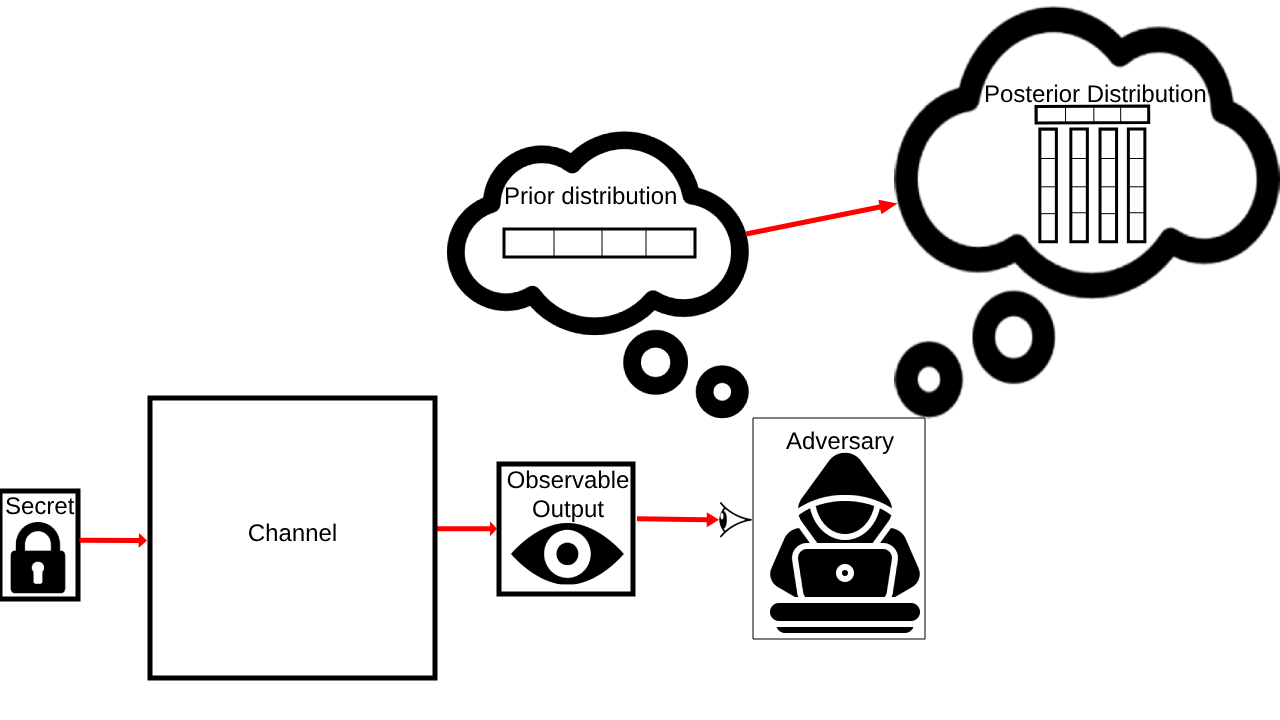
\includegraphics[width=\textwidth]{channelAndFriends}
\caption{Figure representing the scenario we consider in Quantitative Information Flow.}\label{fig:channelAndFriends}
\end{figure*}

We consider the $g$-vulnerability framework, introduced in \cite{QIF}. This framework introduces new definitions, which we present more formally:

\begin{definition}[Gain Function]
A \emph{Gain Function} is a function $g : \mathcal{W} \times \mathcal{X} \rightarrow \mathbb{R}$, such that $g(w,x)$ defines the gain of the adversary if she takes the action $w$ when the secret value is actually $x$. 
\end{definition}

We do not have a loss for the system owner because we consider a zero-sum game: the gain of the adversary is exactly the loss of the people responsible for the system. 

\begin{definition}[Prior g-Vulnerability]
The \emph{Prior Vulnerability} of the system is defined as the average gain of the adversary if she takes the action that maximizes her expected gain, according to the distribution on secrets that represents her prior knowledge. Given a prior distribution on secrets $\pi$ and a gain function $g$, this is defined as:

$$V_g(\pi) = \max\limits_{w\in \mathcal{W}}\sum\limits_{x\in\mathcal{X}} \pi_x g(w,x)$$
\end{definition}

\begin{definition}[Posterior g-Vulnerability]
The \emph{Posterior Vulnerability} of the system is defined in the same way as the prior vulnerability, but considering the hyper-distribution that represents the posterior knowledge. Given a prior distribution on secrets $\pi$ and a channel $C$ and a gain function $g$, this is defined as:

$$V_g[\pi\triangleright C] = \sum\limits_{y \in \mathcal{Y}}\max\limits_{w\in \mathcal{W}}\sum\limits_{x\in\mathcal{X}} \pi_xC_{x,y} g(w,x)$$
\end{definition}

The posterior g-vulnerability represents what will be the expected gain of the adversary after the system runs, but the estimative is made according to the knowledge the adversary has before the system runs

\begin{definition}[Additive Leakage]
The \emph{Additive Leakage} can be defined as the difference between posterior and prior vulnerability:
$$\mathcal{L}_g^+(\pi,C) = V_g[\pi\triangleright C]-V_g(\pi)$$
\end{definition}

\begin{definition}[Multiplicative Leakage]
The \emph{Multiplicative Leakage} is the result of dividing the posterior vulnerability by the prior vulnerability values:
$$\mathcal{L}_g^\times(\pi,C) = \frac{V_g[\pi\triangleright C]}{V_g(\pi)}$$
\end{definition}

There are many valuable theoretical results about channels regarding the relationships between prior and posterior $g$-vulnerabilities. We mention some of these results:

\begin{enumerate}
\item \cite[Chapter~7]{QIF} shows results about the \emph{capacity} of a channel, which is the maximum possible (additive or multiplicative) leakage that can happen through a channel if we fix either the prior, the gain function or neither.
\item \cite[Chapter~9]{QIF} shows results about \emph{refinement} of channels: in short, a channel is strictly better (for all priors and gain functions) than another channel in respect to the posterior vulnerability if and only if it can be written as a post-processing of this other channel.
\item \cite[Chapter~10]{QIF} presents the notion of \emph{Dalenious vulnerability}: it might be the case that the adversary is interested in a secret other than the one considered in the system, and can obtain information about this other system via a known joint distribution between this other secret and the secret that the system considers. In this case, a channel is also strictly better than another in respect to Dalenious leakage, for any such joint distribution and gain function, if and only it can be written as a post-processing of this other channel.
\item \cite[Chapter~11]{QIF} discusses the axiomatic characterization of the notion of vulnerability, and even how some results can be obtained by different axioms that consider the worst-case scenario instead of the average gains of the adversary.
\end{enumerate}

Even though most of the work on Quantitative Information Flow was developed with a stronger focus on measuring how system a system is, the $g$-vulnerability framework can be considered a general notion for quantifying information flow. This means that, in the future, we might be able to use it in the areas explored in this work, as some can be viewed in terms of information flows.
